\begin{activity} \label{8.5.Act3}
\ba
\item Plot the graphs of several of Taylor polynomials centered at 0 (of order at least 5) for $e^x$ and convince yourself that these Taylor polynomials converge to $e^x$ for every value of $x$.
\item Draw the graphs of several of the Taylor polynomials centered at 0 (of order at least 6) for $\cos(x)$ and convince yourself that these Taylor polynomials converge to $\cos(x)$ for every value of $x$. Write the Taylor series centered at 0 for $\cos(x)$.
\item Draw the graphs of several of the Taylor polynomials centered at 0 for $\frac{1}{1-x}$. Based on your graphs, for what values of $x$  do these Taylor polynomials appear converge to $\frac{1}{1-x}$? How is this situation different from what we observe with $e^x$ and $\cos(x)$?  In addition, write the Taylor series centered at 0 for $\frac{1}{1-x}$.
\ea


\end{activity}

\begin{smallhint}
\ba
	\item Small hints for each of the prompts above.
\ea
\end{smallhint}
\begin{bighint}
\ba
	\item Big hints for each of the prompts above.
\ea
\end{bighint}
\begin{activitySolution}
\ba
	\item The graphs of the 10th (magenta), 20th (blue), and 30th (green) Taylor polynomials centered at 0 for $e^x$ are shown below along with the graph of $f(x)$ in red:
\begin{center} \resizebox{!}{1.75in}{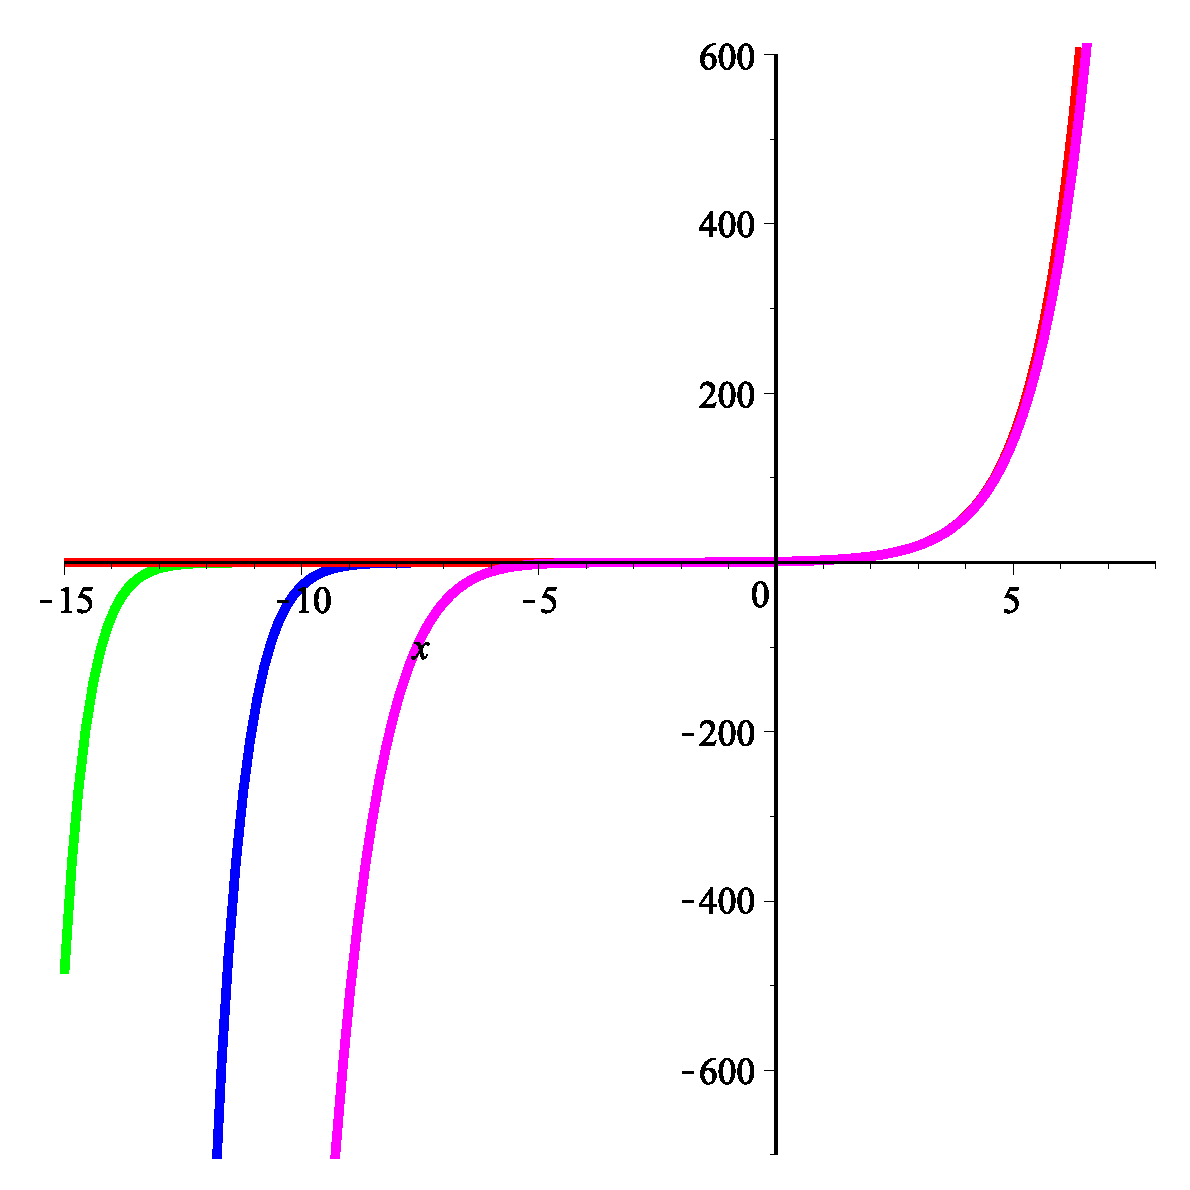
\includegraphics{figures/8_5_exp_graphs.eps}} \end{center} 
It appears that as we increase the order of the Taylor polynomials, they fit the graph of $f$ better and better over larger intervals. So it looks like the Taylor polynomials converge to $e^x$ for every value of $x$. 

\item The graphs of the 10th (magenta), 20th (blue), and 30th (green) Taylor polynomials centered at 0 for $\cos(x)$ are shown below along with the graph of $f(x)$ in red:
\begin{center} \resizebox{!}{1.75in}{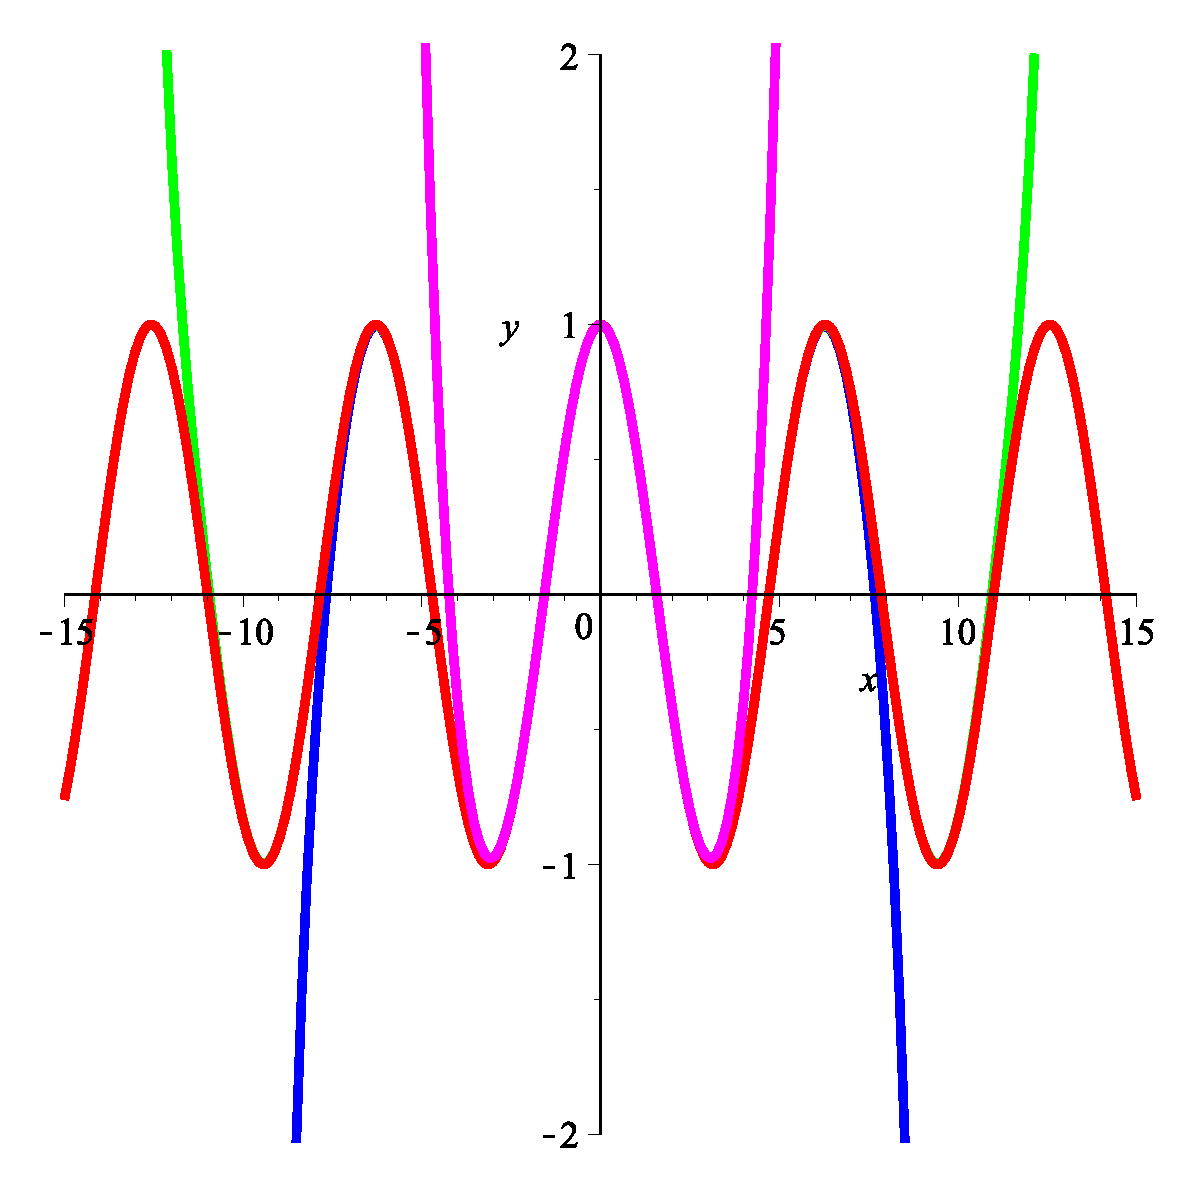
\includegraphics{figures/8_5_cos_graphs.eps}} \end{center}
It appears that as we increase the order of the Taylor polynomials, they fit the graph of $f$ better and better over larger intervals. So it looks like the Taylor polynomials converge to $\cos(x)$ for every value of $x$.
Based on the $n$th order Taylor polynomials we found earlier for $\cos(x)$, the Taylor series for $f(x)$ centered at 0 is
\[\sum_{k=0}^{\infty} \frac{x^{2k}}{(2k)!}.\]

\item The graphs of the 10th (magenta), 20th (blue), and 30th (green) Taylor polynomials centered at 0 for $\frac{1}{1-x}$ are shown below along with the graph of $f(x)$ in red:
\begin{center} \resizebox{!}{1.75in}{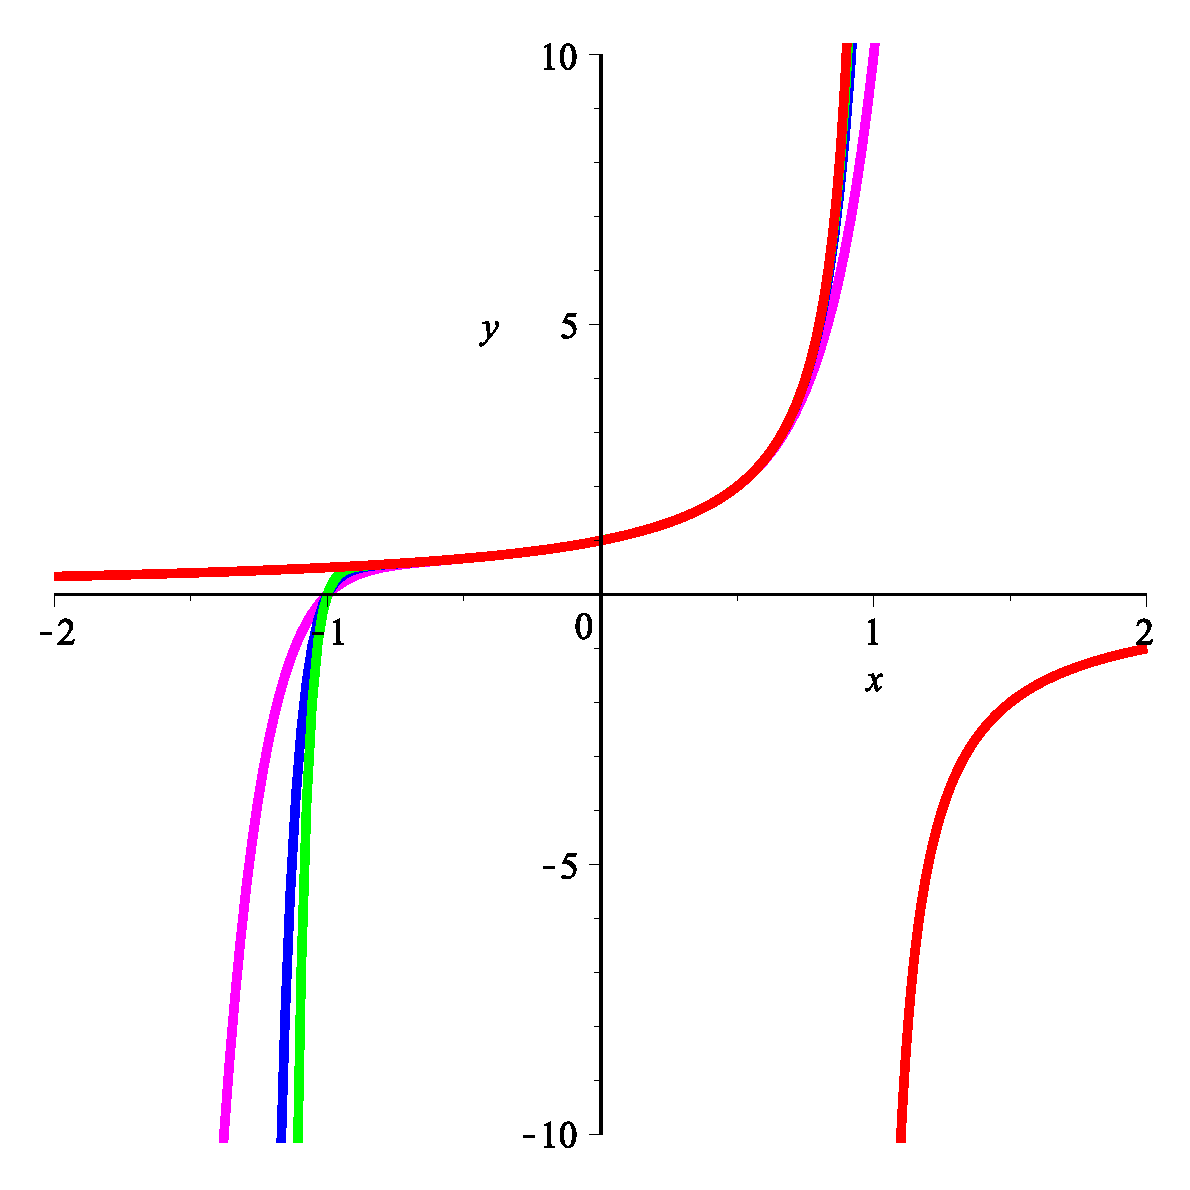
\includegraphics{figures/8_5_1over1minusx_graphs.eps}} \end{center}

It appears that as we increase the order of the Taylor polynomials, they only fit the graph of $f$ better and better over the interval $(-1,1)$ and appear to diverge outside that interval. So it looks like the Taylor polynomials converge to $\frac{1}{1-x}$ only on the interval $(-1,1)$.

Based on the $n$th order Taylor polynomials we found earlier for $\frac{1}{1-x}$, the Taylor series for $f(x)$ centered at 0 is
\[\sum_{k=0}^{\infty} x^k.\]
\ea
\end{activitySolution}
\aftera 